\documentclass[10pt, aspectratio=169]{beamer}

%======================================================
% Theme (matches Lectures 7/8/9/12)
%======================================================
\usetheme[progressbar=frametitle, sectionpage=progressbar, subsectionpage=progressbar, numbering=fraction, block=fill]{metropolis}

\definecolor{mLightBrown}{HTML}{4D4D4D}
\definecolor{mMediumBrown}{HTML}{2C2C2A}
\definecolor{mDarkBrown}{HTML}{1A1A19}
\definecolor{mDarkTeal}{HTML}{0F6E56}
\definecolor{mDarkRed}{HTML}{B03A2E}
\setbeamercolor{normal text}{fg=mDarkBrown}
\setbeamercolor{alerted text}{fg=mDarkTeal}
\setbeamercolor{frametitle}{bg=mDarkBrown}
\setbeamercolor{progress bar}{fg=mDarkTeal, bg=mDarkTeal!20}

\definecolor{mPaleBg}{HTML}{F4F3EE}
\setbeamercolor{block title}{bg=mDarkBrown!10, fg=mDarkBrown}
\setbeamercolor{block body}{bg=mPaleBg, fg=mDarkBrown}
\newcommand{\hl}[1]{\textcolor{mDarkTeal}{#1}}

%======================================================
\usepackage{amsmath, amssymb, amsthm, mathtools}
\usepackage{cancel}
\usepackage{bm}
\usepackage{booktabs}
\usepackage{array}
\usepackage{xcolor}
\usepackage{colortbl}
\usepackage{multirow}
\usepackage{tikz}
\usetikzlibrary{positioning,arrows.meta,calc,fit,shapes.geometric,decorations.pathmorphing}

%======================================================
\newcommand{\paper}[1]{\textcolor{mLightBrown}{\small\textit{(#1)}}}

% --- the recurring four-question strip ---------------
\newcommand{\qcur}{0}
\newcommand{\qnode}[4]{%
\ifnum#4=\qcur
 \node[draw=mDarkTeal, fill=mDarkTeal!12, thick, rounded corners=1pt, minimum width=3.0cm, minimum height=0.52cm, font=\tiny\bfseries, text=mDarkBrown] (#2) at (#1,0) {#3};%
\else
 \node[draw=mLightBrown!45, rounded corners=1pt, minimum width=3.0cm, minimum height=0.52cm, font=\tiny, text=mLightBrown] (#2) at (#1,0) {#3};%
\fi}
\newcommand{\qstrip}[1]{\renewcommand{\qcur}{#1}%
\begin{center}
\begin{tikzpicture}
\qnode{0}{q1}{Q1 Gradient?}{1}
\qnode{3.7}{q2}{Q2 Variance?}{2}
\qnode{7.4}{q3}{Q3 Continuous?}{3}
\qnode{11.1}{q4}{Q4 Safe step?}{4}
\draw[-{Stealth}, mLightBrown!60] (q1.east) -- (q2.west);
\draw[-{Stealth}, mLightBrown!60] (q2.east) -- (q3.west);
\draw[-{Stealth}, mLightBrown!60] (q3.east) -- (q4.west);
\end{tikzpicture}\end{center}}

%======================================================
\title{Policy-Based Reinforcement Learning}
\subtitle{Optimal control with the dynamics replaced by data}
\author{Jinkyoo Park}
\institute{KAIST}
\date{\textit{Lecture 10 --- The data-driven extension of the control-theory lineage}}

%======================================================
\begin{document}
%======================================================

\maketitle

%==========================================================
\section{The handoff --- delete the dynamics}
%==========================================================

\begin{frame}{Where we are --- the lineage completes}
\vspace{2pt}
\begin{center}\footnotesize
\renewcommand{\arraystretch}{1.35}
\begin{tabular}{r|c|c}
 & \textbf{OR / Dynamic Programming} & \textbf{Control Theory} \\
\hline
\textbf{Model-based (origin)}  & MDP \& DP \scriptsize(Lec.\ 7) & Optimal Control \scriptsize(Lec.\ 9)\\
\hline
\textbf{Data-driven (extension)} & Value-Based RL \scriptsize(Lec.\ 8) & \cellcolor{mDarkTeal!20}\textbf{Policy-Based RL} \scriptsize(\alert{Lec.\ 10})\\
\end{tabular}
\end{center}
\smallskip

The map closes with a clean symmetry --- one move, applied to each parent:
\begin{itemize}\setlength\itemsep{1pt}
\item Lecture 8: \emph{MDP/DP is the OR origin; \alert{delete the model $(P,R)$} $\Rightarrow$ value-based RL.}
\item Lecture 10: \emph{Optimal control is the control origin; \alert{delete the dynamics $f$} $\Rightarrow$ policy-based RL.}
\end{itemize}
\medskip

\pause
So this lecture is \alert{Lecture 9, with $f$ taken away and replaced by samples}. Where optimal control \emph{solved} the dynamics for a feedback law $u=\gamma(t,x)$, we will \emph{learn} that law $\pi_\theta(a\mid s)$ directly from data.
\end{frame}

\begin{frame}{Two reasons to learn the policy directly}
The fixed point of this lecture, in one line:
\begin{center}\large
\alert{When you cannot solve for the controller, learn to output it.}
\end{center}
\medskip

\pause
Two independent pressures both demand a \emph{directly parameterized policy}:
\begin{itemize}\setlength\itemsep{3pt}
\item \textbf{From the control side (the lineage):} the optimal-control solvers --- HJB, Riccati, Pontryagin --- all needed $f$. With only data, we cannot run them. So parameterize $\pi_\theta$ and improve it from samples.
\item \textbf{From the value side (the wall):} Lecture 8's methods chose actions by $\arg\max_a Q(s,a)$. In continuous control that maximization is itself intractable. A parameterized policy \alert{outputs} the action --- no search.
\end{itemize}
\medskip

\pause
Both arrive at the same object: a controller $\pi_\theta$ improved by gradient ascent on expected return. The control lineage gives it meaning (a learned feedback law); the value wall gives it urgency (continuous actions).
\end{frame}

\begin{frame}{The translation table --- optimal control, learned}
Every object of Lecture 9 has a data-driven counterpart.
\medskip
\begin{center}\scriptsize\renewcommand{\arraystretch}{1.55}
\begin{tabular}{l|l|l}
\textbf{Lecture 9 (optimal control)} & \textbf{Lecture 10 (policy-based RL)} & \textbf{What replaces the model} \\
\hline
value field $V(t,x)$, HJB & critic $V_w,\,Q_w$ & a learned value \\
feedback law $u=\gamma(t,x)$, $u=Kx$ & actor $\pi_\theta(a\mid s)$ / $\mu_\theta(s)$ & a learned controller \\
known dynamics $\dot x = f(x,u)$ & sampled transitions $(s,a,r,s')$ & the environment \\
Pontryagin costate / trajectory opt.\ & REINFORCE / trajectory sampling & the score-function trick \\
solve Riccati / HJB & gradient ascent on $J(\theta)$ & stochastic optimization \\
\end{tabular}
\end{center}
\medskip

\pause
\begin{center}\large
\alert{Policy gradient is optimal control with $f$ deleted and replaced by data.}
\end{center}
DDPG's actor $\mu_\theta(s)$ is the learned cousin of LQR's gain $K$; REINFORCE is Pontryagin's trajectory view with the dynamics sampled rather than known.
\end{frame}

\begin{frame}{The roadmap --- four questions}
One question per Act. This strip returns at every transition.
\qstrip{0}
\medskip
\begin{itemize}\setlength\itemsep{3pt}
\item \textbf{Q1 --- How do we get a gradient without $f$?} The \alert{score-function trick} --- the dynamics vanish. \paper{Williams 1992; Sutton et al., 2000}
\item \textbf{Q2 --- Why is it so noisy?} Baselines, advantage, and the \alert{actor--critic}. \paper{Mnih et al., 2016}
\item \textbf{Q3 --- How do we handle continuous control?} \alert{DPG / DDPG} --- the actor climbs $\nabla_a Q$. \paper{Silver 2014; Lillicrap 2015}
\item \textbf{Q4 --- How do we step without falling?} Trust regions: \alert{TRPO} and \alert{PPO}. \paper{Schulman et al., 2015; 2017}
\end{itemize}
\end{frame}

%==========================================================
\section{Act 1 --- a gradient without the model}
%==========================================================

\begin{frame}{The objective, and a gradient we cannot see}
\qstrip{1}
\medskip
Parameterize a stochastic policy $\pi_\theta(a\mid s)$; maximize expected return:
\[
J(\theta) = \mathbb{E}_{\tau\sim\pi_\theta}\big[R(\tau)\big], \qquad \theta \leftarrow \theta + \alpha\,\nabla_\theta J(\theta).
\]
The trajectory's probability \emph{contains the unknown dynamics}:
\[
p_\theta(\tau) = \mu(s_0)\prod_{t} \pi_\theta(a_t\mid s_t)\,\hl{P(s_{t+1}\mid s_t,a_t)}.
\]
\medskip

\pause
This is the data-driven echo of Lecture 9's predicament: there, $f$ was known and we solved; here $P$ is \alert{unknown} and inside the very distribution we must differentiate. How can we take the gradient of an expectation whose law we cannot see?
\end{frame}

\begin{frame}{The score-function trick --- the dynamics vanish}
The identity $\nabla p = p\,\nabla\log p$ turns gradient-of-expectation into expectation-of-gradient:
\[
\nabla_\theta J = \mathbb{E}_{\tau\sim\pi_\theta}\big[\nabla_\theta\log p_\theta(\tau)\,R(\tau)\big].
\]
Now expand $\log p_\theta(\tau)$ --- the model terms carry no $\theta$ and die:
\[
\nabla_\theta \log p_\theta(\tau) = \nabla_\theta\Big[\cancel{\log\mu(s_0)} + \sum_t \log\pi_\theta(a_t\mid s_t) + \cancel{\textstyle\sum_t \log P(s_{t+1}\mid s_t,a_t)}\Big] = \sum_t \nabla_\theta\log\pi_\theta(a_t\mid s_t).
\]
\medskip

\pause
\begin{center}\large
\alert{The start distribution and the dynamics contribute exactly zero to the gradient.}
\end{center}
This is the precise sense in which $f$ is ``deleted'': we never needed it. Where Lecture 9 \emph{solved} the dynamics, here they simply drop out of the math --- the policy's own log-probability is all that remains.
\end{frame}

\begin{frame}{The policy gradient theorem --- and REINFORCE}
Cleaning up (the DP-based derivation, Backup 1) gives the canonical form:
\[
\nabla_\theta J(\theta) = \mathbb{E}_{\pi_\theta}\big[\,\nabla_\theta \log \pi_\theta(a\mid s)\; Q^{\pi_\theta}(s,a)\,\big].
\]
\textbf{Reading it.} Push up the log-probability of each action, \alert{weighted by how good it was}. Good actions become more likely, bad ones less --- reweighted imitation of one's own better moments. No $\arg\max$, no model.
\medskip

\pause
\textbf{REINFORCE} makes it runnable by replacing $Q^\pi$ with the sampled return $G_t$:
\[
\theta \leftarrow \theta + \alpha \sum_t \nabla_\theta \log\pi_\theta(a_t\mid s_t)\, G_t.
\]
Unbiased (since $\mathbb{E}_\pi[G_t\mid s,a]=Q^\pi$), but Monte-Carlo --- so \alert{unbiased and high variance}. Taming that variance is Act 2.
\end{frame}

%==========================================================
\section{Act 2 --- taming variance with a critic}
%==========================================================

\begin{frame}{Baselines --- subtract anything action-independent}
\qstrip{2}
\medskip
Subtract a state-dependent baseline $b(s)$:
\[
\nabla_\theta J = \mathbb{E}_{\pi_\theta}\big[\nabla_\theta\log\pi_\theta(a\mid s)\,(Q^\pi(s,a) - b(s))\big].
\]
\begin{block}{The baseline is free \hfill {\scriptsize\normalfont it adds \emph{zero} bias}}
\centering
$\mathbb{E}_{a\sim\pi}\big[\nabla_\theta\log\pi_\theta(a\mid s)\,b(s)\big] = b(s)\,\nabla_\theta\!\sum_a \pi_\theta(a\mid s) = b(s)\,\nabla_\theta 1 = 0.$
\end{block}
\medskip

\pause
The natural choice $b(s)=V^\pi(s)$ leaves the \alert{advantage}:
\[
A^\pi(s,a) = Q^\pi(s,a) - V^\pi(s) \quad\text{--- ``how much better than average is this action?''}
\]
The gradient now pushes on actions \emph{relative} to the state's baseline value --- same mean, far less variance. We just created a need for a learned $V$: the critic.
\end{frame}

\begin{frame}{Actor--critic --- a learned value steadies the policy}
Learn both: an \textbf{actor} $\pi_\theta$ and a \textbf{critic} $V_w$ supplying the advantage.
\medskip
\begin{center}
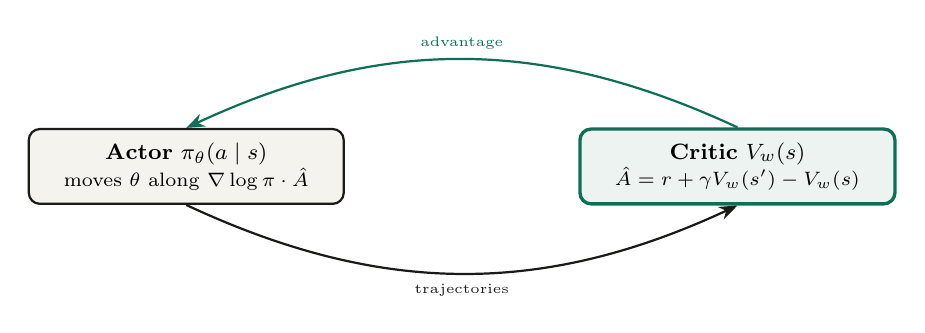
\begin{tikzpicture}[font=\footnotesize, node distance=10pt]
\node[draw=mDarkBrown, thick, fill=mPaleBg, rounded corners, minimum width=4.0cm, minimum height=0.95cm, align=center] (actor) at (0,0) {\textbf{Actor} $\pi_\theta(a\mid s)$\\ \scriptsize moves $\theta$ along $\nabla\log\pi\cdot \hat A$};
\node[draw=mDarkTeal, very thick, fill=mDarkTeal!8, rounded corners, minimum width=4.0cm, minimum height=0.95cm, align=center] (critic) at (7,0) {\textbf{Critic} $V_w(s)$\\ \scriptsize $\hat A = r + \gamma V_w(s') - V_w(s)$};
\draw[-{Stealth}, mDarkTeal, thick] (critic.north) to[bend right=25] node[above,font=\tiny]{advantage} (actor.north);
\draw[-{Stealth}, mDarkBrown, thick] (actor.south) to[bend right=25] node[below,font=\tiny]{trajectories} (critic.south);
\end{tikzpicture}
\end{center}
\medskip

\pause
The critic's $\hat A$ is a TD error --- \alert{value-based RL (Lecture 8) living inside the policy update}. Here the two lineages briefly touch: a control-lineage actor steadied by an OR-lineage critic.
\medskip
\begin{itemize}\setlength\itemsep{1pt}
\item \textbf{A2C / A3C} --- parallel actors decorrelate data (replacing the replay buffer). \paper{Mnih et al., 2016}
\item \textbf{GAE} --- a $\lambda$-dial trading the advantage's bias against variance. \paper{Schulman et al., 2016}
\end{itemize}
\end{frame}

%==========================================================
\section{Act 3 --- continuous control: DDPG}
%==========================================================

\begin{frame}{The continuous fix --- deterministic policy gradient}
\qstrip{3}
\medskip
For continuous actions, make the actor \alert{deterministic}, $a=\mu_\theta(s)$, and let it climb the critic's action-gradient:
\[
\nabla_\theta J(\mu_\theta) = \mathbb{E}_{s\sim\rho}\Big[\,\nabla_\theta \mu_\theta(s)\; \nabla_a Q(s,a)\big|_{a=\mu_\theta(s)}\Big]. \qquad \paper{Silver et al., 2014}
\]
\medskip
\begin{center}\large
\alert{This is how the intractable $\max_a Q$ is finally beaten:} the actor follows $\nabla_a Q$ uphill, instead of searching.
\end{center}
\medskip

\pause
\textbf{DDPG} \paper{Lillicrap et al., 2015} $=$ DPG $+$ all of DQN's stabilizers:
\begin{itemize}\setlength\itemsep{1pt}
\item off-policy critic by Bellman error; \emph{replay buffer} and \emph{target networks} (the deadly-triad fixes from Lecture 8 return);
\item temporally-correlated \alert{Ornstein--Uhlenbeck} exploration --- a deterministic actor explores nothing on its own.
\end{itemize}
\end{frame}

\begin{frame}{$\mu_\theta(s)$ is the learned $K$ --- the lineage made literal}
Put Lecture 9 and this slide side by side.
\medskip
\begin{center}\footnotesize\renewcommand{\arraystretch}{1.4}
\begin{tabular}{l|c|c}
 & \textbf{LQR (Lecture 9)} & \textbf{DDPG (here)} \\
\hline
the controller & $u = -Kx$ & $a = \mu_\theta(s)$ \\
how obtained & solve the Riccati equation & ascend $\nabla_a Q$ from samples \\
needs the model? & yes ($A,B$) & \alert{no} (sampled transitions) \\
form & a matrix & a neural network \\
\end{tabular}
\end{center}
\medskip

\pause
\begin{center}\large
Same feedback law, two ways to find it: \alert{solve the dynamics, or sample their gradient.}
\end{center}
This is the whole two-lineage story in one comparison --- the model-based controller of the control tradition, and its data-driven twin.
\end{frame}

%==========================================================
\section{Act 4 --- stepping without falling}
%==========================================================

\begin{frame}{The step-size trap unique to RL}
\qstrip{4}
\medskip
In supervised learning a bad step costs one bad update. In RL it is worse:
\begin{center}\large
\alert{the policy generates its own next batch of data.}
\end{center}
A step that pushes $\pi_\theta$ too far lands in a region where the policy is terrible --- and now \emph{all} subsequent data comes from that terrible policy. The damage is self-reinforcing.
\medskip

\pause
So we want the largest improving step that keeps the new policy \alert{close to the old one in behavior} --- measured by KL divergence between action distributions, not by distance in parameters. A \emph{trust region in policy space} is the last piece.
\end{frame}

\begin{frame}{TRPO and PPO --- the trust region, exact and cheap}
\textbf{TRPO} maximizes an importance-weighted advantage inside a KL ball \paper{Schulman et al., 2015}:
\[
\max_{\theta}\; \mathbb{E}\!\left[\frac{\pi_\theta(a\mid s)}{\pi_{\theta_{\text{old}}}(a\mid s)}\,\hat A\right]
\;\text{ s.t. }\;
\mathbb{E}\big[D_{\mathrm{KL}}(\pi_{\theta_{\text{old}}}\,\|\,\pi_\theta)\big] \le \delta
\;\Rightarrow\; \text{\alert{monotonic improvement}}.
\]
Solved by a natural-gradient step (linearize objective, quadratize KL via Fisher). Powerful but heavy.
\medskip

\pause
\textbf{PPO} keeps the intent with a \alert{clipped surrogate} --- no second-order machinery \paper{Schulman et al., 2017}:
\[
J^{\text{CLIP}}(\theta) = \mathbb{E}\Big[\min\big(\,r(\theta)\,\hat A,\ \mathrm{clip}(r(\theta),1-\epsilon,1+\epsilon)\,\hat A\,\big)\Big], \quad r(\theta)=\tfrac{\pi_\theta}{\pi_{\theta_{\text{old}}}}.
\]
When the ratio leaves $[1-\epsilon,1+\epsilon]$, the clip removes the incentive to push further --- a soft trust region for free.
\medskip
\pause
\begin{center}\large
PPO is the default workhorse of modern policy-based RL.
\end{center}
\end{frame}

%==========================================================
\section{Closing}
%==========================================================

\begin{frame}{Where we are --- both lineages, now data-driven}
\vspace{2pt}
\begin{center}\footnotesize
\renewcommand{\arraystretch}{1.35}
\begin{tabular}{r|c|c}
 & \textbf{OR / Dynamic Programming} & \textbf{Control Theory} \\
\hline
\textbf{Model-based} & MDP \& DP \;{\scriptsize Lec.\ 7 \checkmark} & Optimal Control \;{\scriptsize Lec.\ 9 \checkmark}\\
\hline
\textbf{Data-driven} & Value-Based RL \;{\scriptsize Lec.\ 8 \checkmark} & \cellcolor{mDarkTeal!15}\textbf{Policy-Based RL} \;{\scriptsize Lec.\ 10 \checkmark}\\
\end{tabular}
\end{center}
\medskip

\pause
The 2$\times$2 is complete. Two traditions, each with a model-based origin and a data-driven extension, related by the same move: \;\textbf{delete the model, sample instead.}
\medskip

\pause
\begin{center}\large
What is left is to \alert{put the model back} --- but learned. That reunion is Lecture 11.
\end{center}
\end{frame}

\begin{frame}{Closing --- the one sentence}
\vfill
\begin{center}\large
Optimal control found the feedback law by solving the dynamics.\\[8pt]
Policy-based RL finds \alert{the same law} by sampling its gradient ---\\[4pt]
the dynamics never solved, only experienced,\\[4pt]
and the controller learned, not derived.
\end{center}
\vfill
\pause
\footnotesize
Read against Lecture 8's closing, the symmetry is exact: value-based RL kept the Bellman equation and threw away the model; policy-based RL kept the feedback law and threw away the dynamics. Two parents, one orphaning move. Lecture 11 learns the model back and lets the two reunite.
\end{frame}

\begin{frame}[standout]
Questions?
\end{frame}

%==========================================================
\appendix
%==========================================================

\begin{frame}{Backup 1 --- the policy gradient theorem}
\footnotesize
Objective $J(\theta)=\sum_s d^\pi(s)V^\pi(s)$, $d^\pi$ the on-policy stationary distribution. Differentiate $V^\pi(s)=\sum_a\pi_\theta(a\mid s)Q^\pi(s,a)$:
\[
\nabla_\theta V^\pi(s) = \sum_a \big[\nabla_\theta\pi_\theta(a\mid s)\,Q^\pi(s,a) + \pi_\theta(a\mid s)\,\nabla_\theta Q^\pi(s,a)\big].
\]
Expand $Q^\pi=\sum_{s'}P(s'\mid s,a)[r+\gamma V^\pi(s')]$; only $V^\pi(s')$ carries $\theta$, giving a recursion. Unrolling and collecting via the $k$-step visitation $\rho^\pi(s\to x,k)$:
\[
\nabla_\theta J = \sum_s d^\pi(s)\sum_a \nabla_\theta\pi_\theta(a\mid s)\,Q^\pi(s,a)
= \mathbb{E}_{\pi}\big[\nabla_\theta\log\pi_\theta(a\mid s)\,Q^\pi(s,a)\big]. \quad\blacksquare
\]
\textbf{Trajectory view (Act 1):} the same result via $\nabla_\theta J=\mathbb{E}_\tau[(\sum_t\nabla_\theta\log\pi_\theta(a_t\mid s_t))R(\tau)]$ --- the dynamics drop because $\nabla_\theta\log P=0$.
\end{frame}

\begin{frame}{Backup 2 --- TRPO's closed-form natural-gradient step}
\footnotesize
$\max_\theta L(\theta):=\mathbb{E}[r(\theta)\hat A]$ s.t. $\bar D_{\mathrm{KL}}(\theta_{\text{old}},\theta)\le\delta$, $r(\theta)=\pi_\theta/\pi_{\theta_{\text{old}}}$.
\medskip

\textbf{Step 1 --- local models.} $L(\theta)\approx g^\top(\theta-\theta_{\text{old}})$, $\bar D_{\mathrm{KL}}\approx\tfrac12(\theta-\theta_{\text{old}})^\top H(\theta-\theta_{\text{old}})$, with $g=\nabla_\theta L$, $H$ the Fisher matrix.
\medskip

\textbf{Step 2 --- linear objective on an ellipsoid.} Optimum along the natural-gradient direction $H^{-1}g$, scaled to KL-radius $\delta$:
\[
\theta_{\text{new}} = \theta_{\text{old}} + \sqrt{\tfrac{2\delta}{\,g^\top H^{-1}g\,}}\,H^{-1}g.
\]
\textbf{Step 3 --- practice.} $H^{-1}g$ by conjugate gradient (never form $H$), backtrack until the true KL/improvement hold. \alert{PPO} discards all of this, recovering the effect with one clip on $r(\theta)$. This trust-region machinery returns verbatim as multi-agent HATRPO in Lecture 12.
\end{frame}

\begin{frame}{Backup 3 --- the policy-based zoo, placed}
\footnotesize
Each method is one cell of: \emph{stochastic vs.\ deterministic actor} $\times$ \emph{on- vs.\ off-policy} $\times$ \emph{variance/step control}.
\medskip
\begin{center}\scriptsize\renewcommand{\arraystretch}{1.4}
\begin{tabular}{l|l|l}
\textbf{Method} & \textbf{Key idea} & \textbf{Reference} \\
\hline
REINFORCE & MC policy gradient, no critic & Williams, 1992 \\
A3C / A2C & parallel actor--critic, advantage & Mnih et al., 2016 \\
GAE & $\lambda$-weighted advantage & Schulman et al., 2016 \\
DPG / DDPG & deterministic actor climbs $\nabla_a Q$; off-policy & Silver 2014; Lillicrap 2015 \\
TD3 & twin critics + delayed actor (overestimation fix) & Fujimoto et al., 2018 \\
TRPO & KL trust region, monotonic improvement & Schulman et al., 2015 \\
PPO & clipped surrogate, the workhorse & Schulman et al., 2017 \\
SAC & maximum-entropy off-policy actor--critic & Haarnoja et al., 2018 \\
\end{tabular}
\end{center}
\medskip
\textbf{Through-line.} All share $\mathbb{E}[\nabla_\theta\log\pi_\theta\,\hat A]$ (or its deterministic $\nabla_a Q$ form); they differ only in \emph{which advantage they trust} (Act 2) and \emph{how large a step they dare} (Act 4). SAC's entropy term is the bridge to Lecture 12's QRE.
\end{frame}

\end{document}
